\section{使用技巧}
\label{section_skills}

\subsection{开机自启罗技软件}
\label{subsection-auto-start-lghub-as-admin}

罗技软件需要\textbf{\color{red}以管理员权限启动},罗技软件自带的开机自启功能无法做到这一点。较为便捷的方式是使用 Windows 自带的\textbf{“任务计划程序”}。

\begin{figure}[H]
    \Centering
    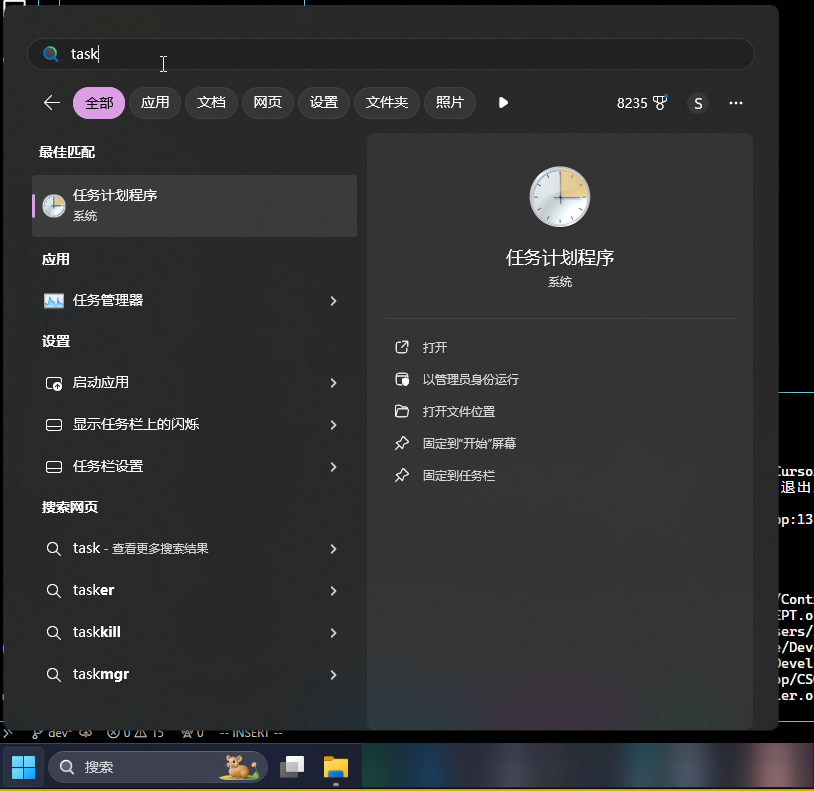
\includegraphics[width=\textwidth]{docs/assets/skills/task_scheduler.png}
    \caption{在开始菜单中搜索“task”,找到“任务计划程序”}
\end{figure}

打开后,右键“任务计划程序库”,点击“新文件夹”创建新文件夹,并为其指定名称。

\begin{figure}[H]
    \Centering
    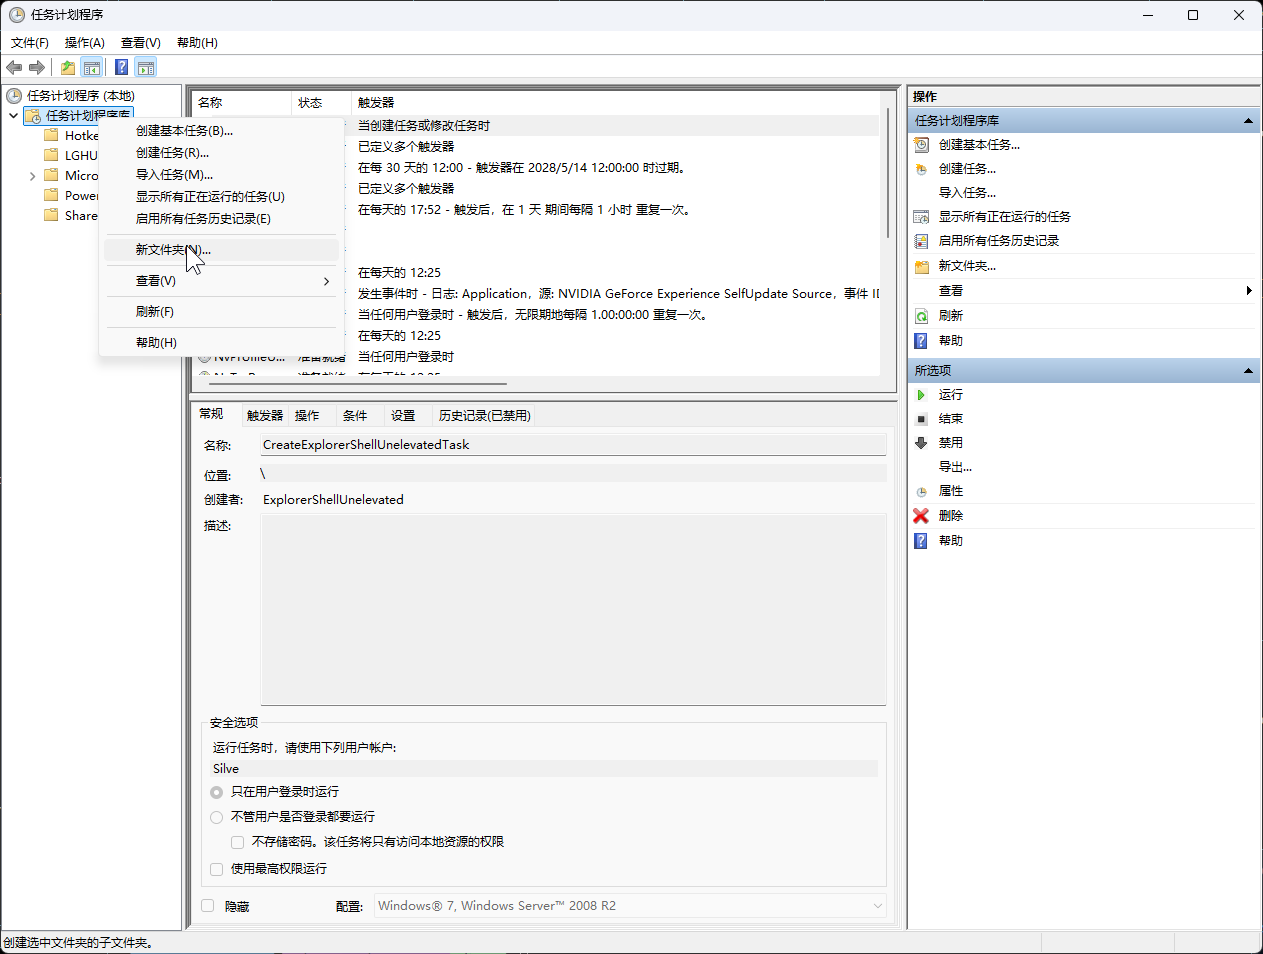
\includegraphics[width=\textwidth]{docs/assets/skills/new_folder.png}
    \caption{点击“新文件夹”}
\end{figure}

\begin{figure}[H]
    \Centering
    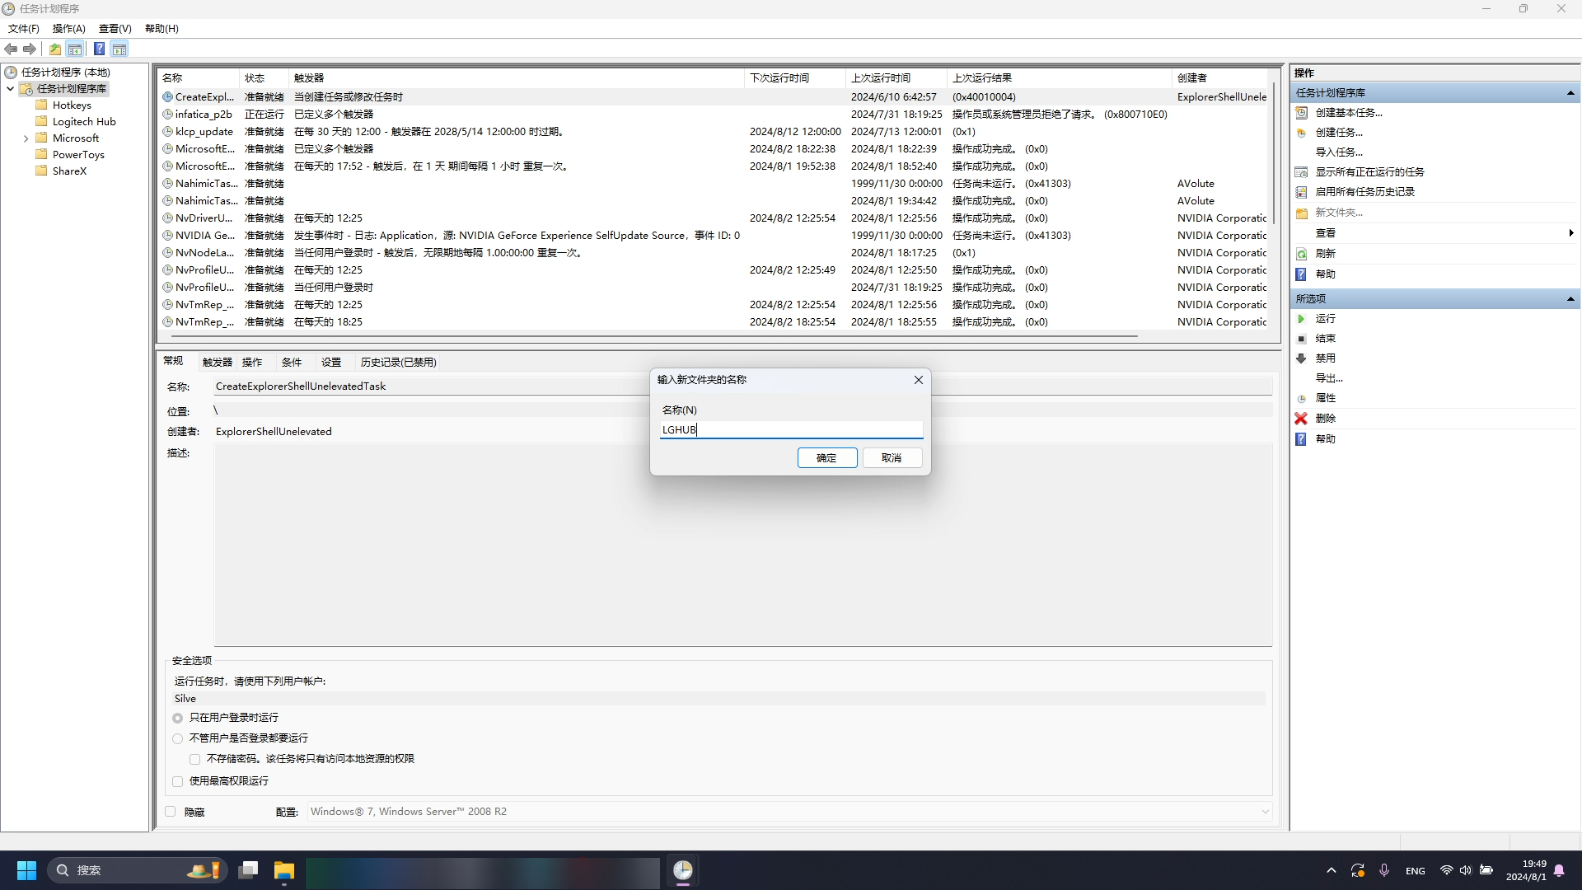
\includegraphics[width=\textwidth]{docs/assets/skills/specify_name.png}
    \caption{指定文件夹名称}
\end{figure}

右键新创建的文件夹,点击“创建基本任务”。

\begin{figure}[H]
    \Centering
    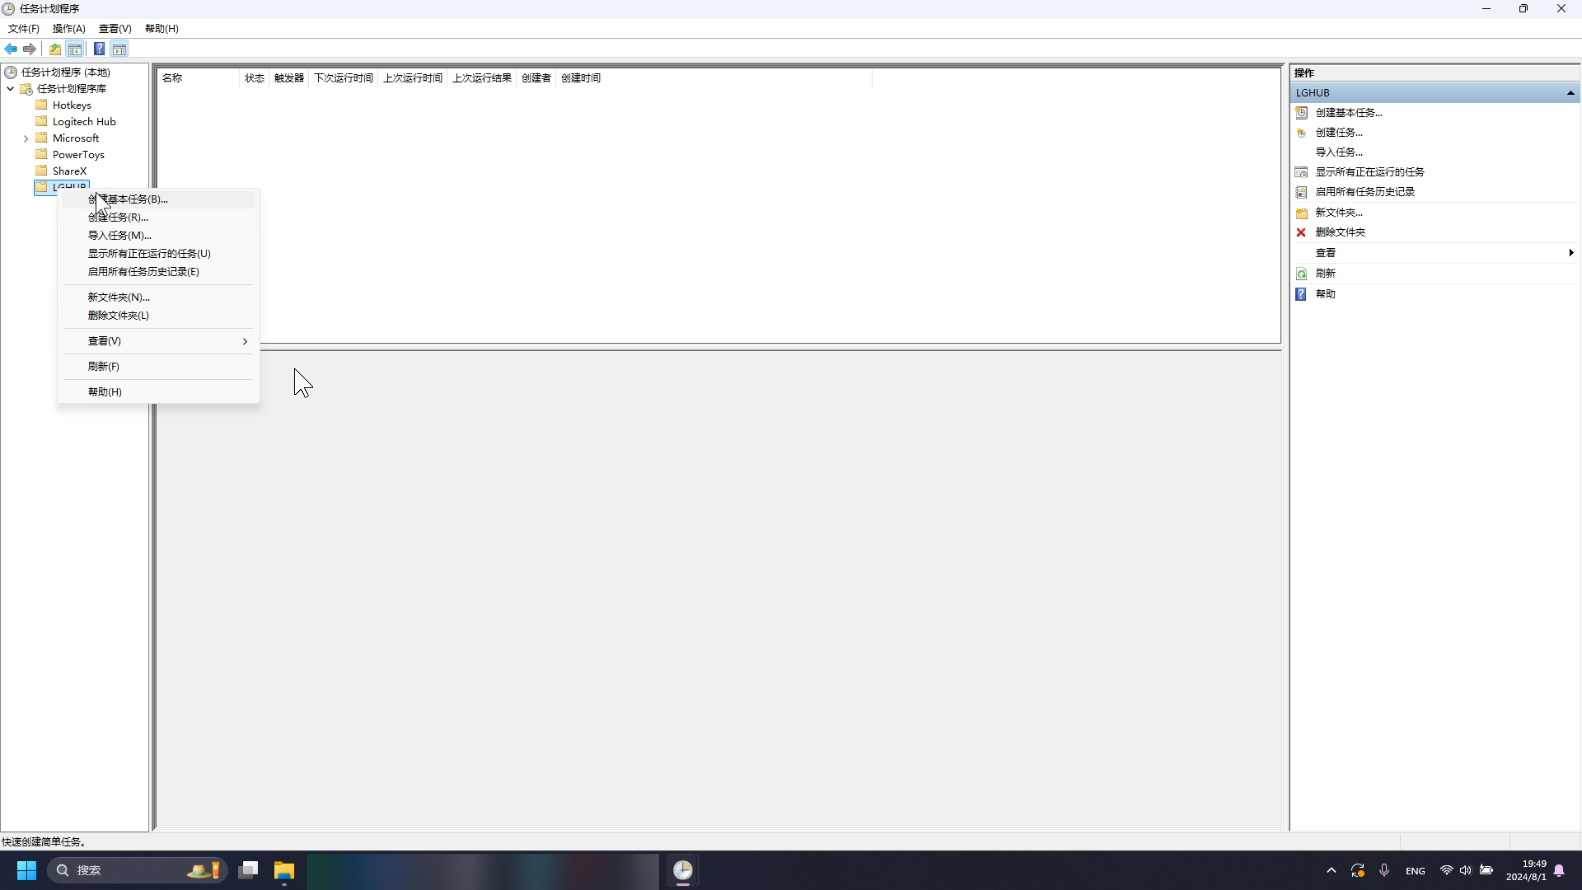
\includegraphics[width=\textwidth]{docs/assets/skills/create_basic_task_00.png}
    \caption{创建基本任务}
\end{figure}

为基本任务设置名称。

\begin{figure}[H]
    \Centering
    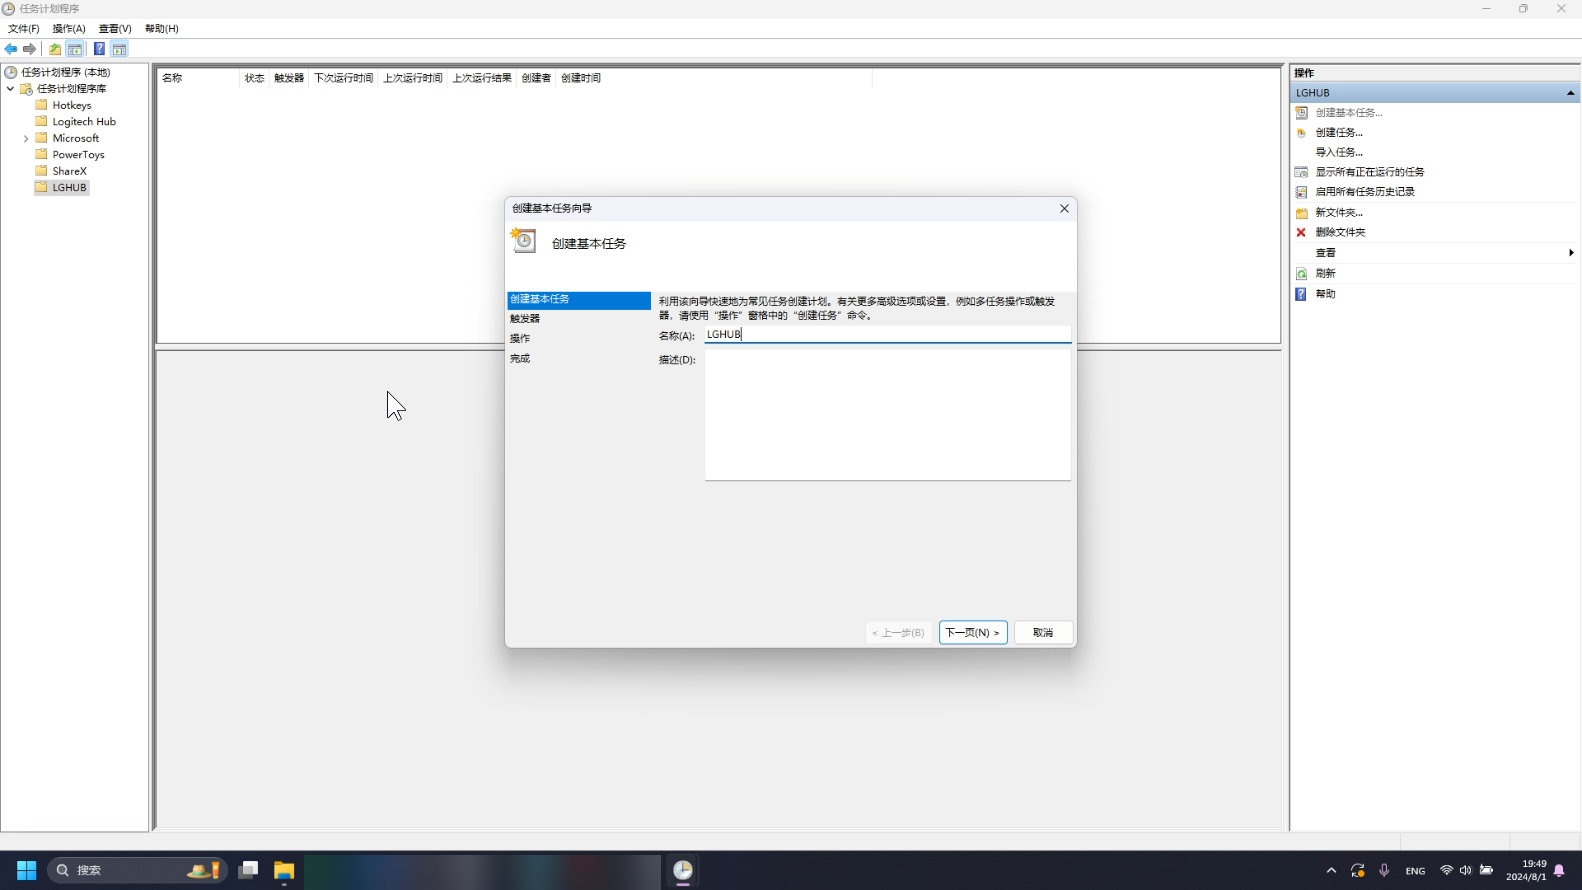
\includegraphics[width=\textwidth]{docs/assets/skills/create_basic_task_01.png}
    \caption{设置基本任务名称}
\end{figure}

触发器中设置任务在“当前用户登录时”开始。

\begin{figure}[H]
    \Centering
    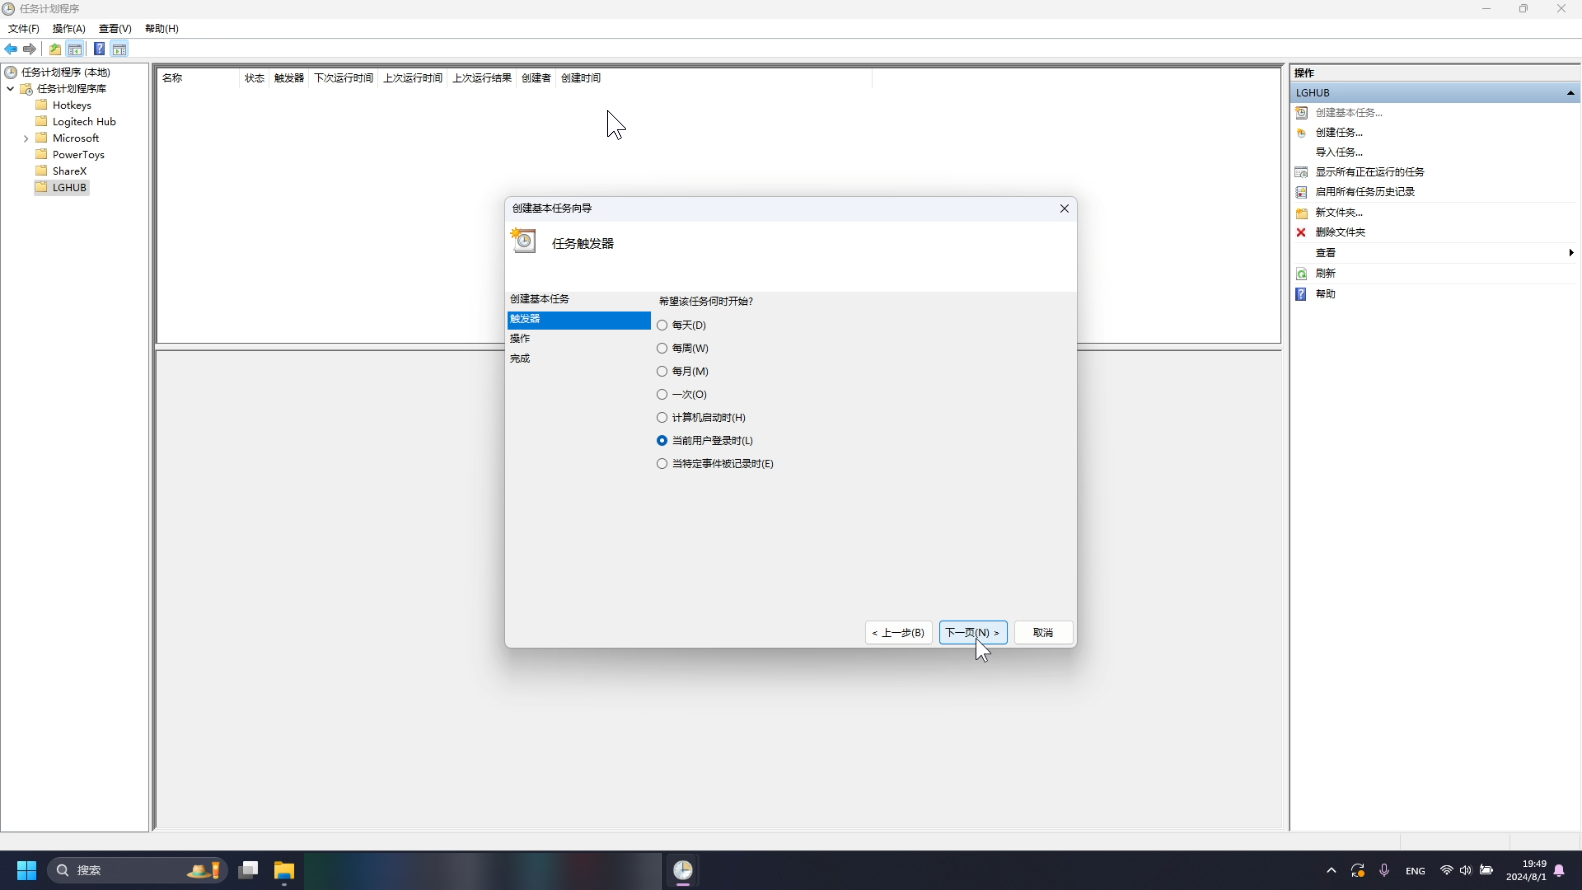
\includegraphics[width=\textwidth]{docs/assets/skills/create_basic_task_02.png}
    \caption{设置触发器}
\end{figure}

执行操作的类型为“启动程序”。

\begin{figure}[H]
    \Centering
    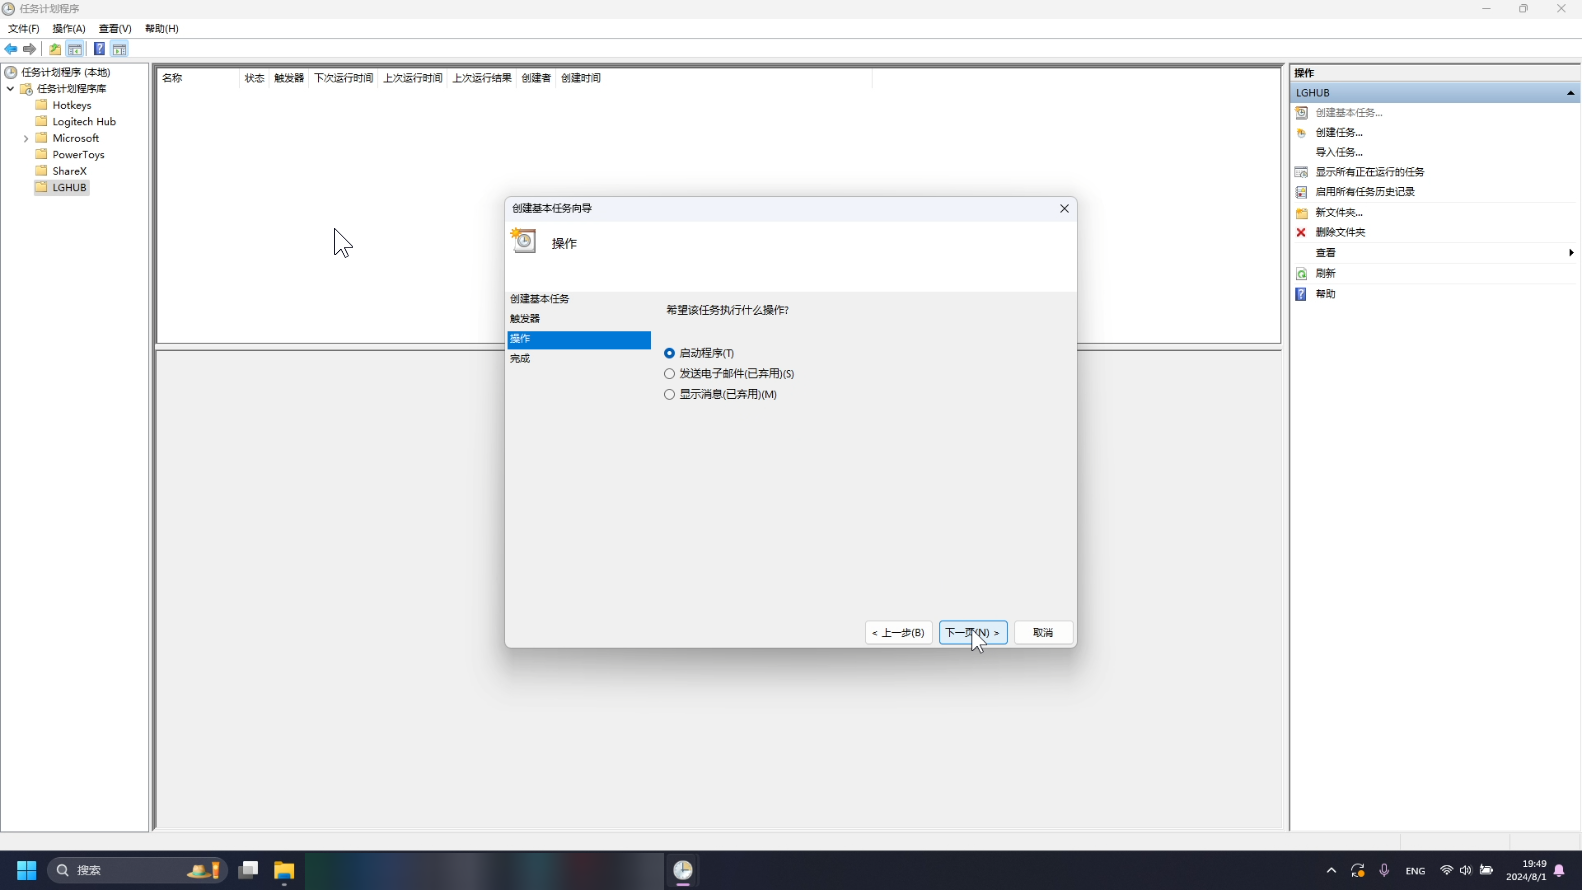
\includegraphics[width=\textwidth]{docs/assets/skills/create_basic_task_03.png}
    \caption{设置操作类型}
\end{figure}
 
然后,在桌面上右键罗技软件快捷方式,点击“属性”。

\begin{figure}[H]
    \Centering
    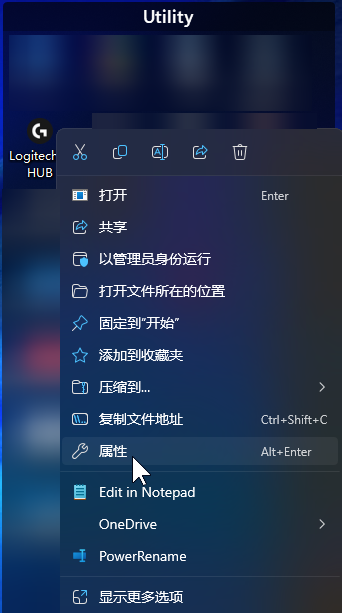
\includegraphics[width=\textwidth]{docs/assets/skills/lghub_property.png}
    \caption{点击“属性”}
\end{figure}

复制快捷方式指向的目标路径到剪切板中(\lstinline{Ctrl} \lstinline{C})。

\begin{figure}[H]
    \Centering
    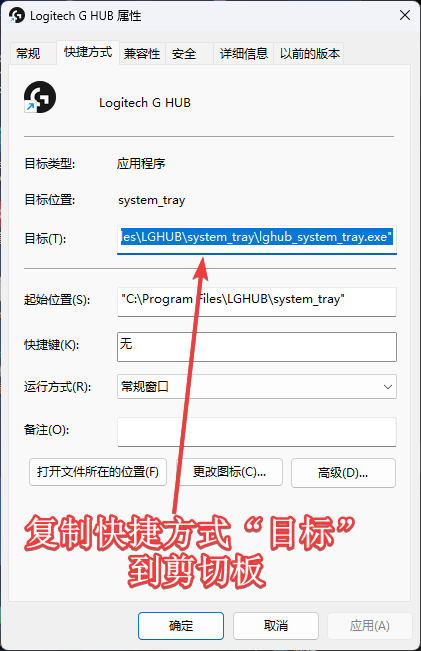
\includegraphics[width=\textwidth]{docs/assets/skills/create_basic_task_04.png}
    \caption{复制快捷方式“目标”}
\end{figure}

在“程序或脚本”一栏粘贴上述步骤复制的目标路径到地址栏(\lstinline{Ctrl} \lstinline{V})。

\begin{figure}[H]
    \Centering
    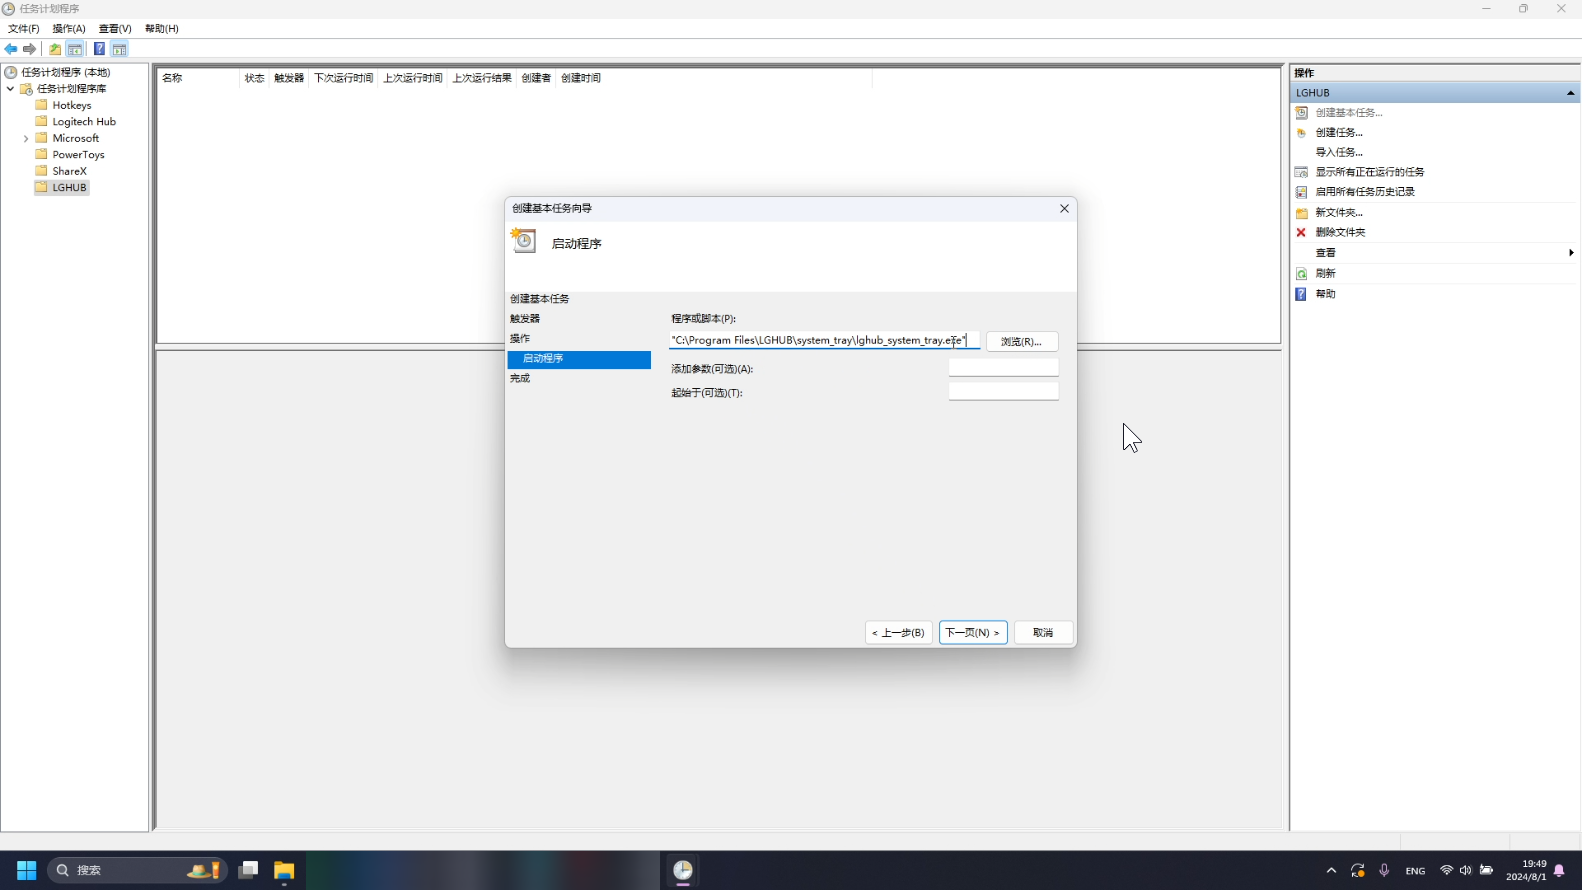
\includegraphics[width=\textwidth]{docs/assets/skills/create_basic_task_05.png}
    \caption{粘贴到地址栏中}
\end{figure}

在添加参数一栏输入 \lstinline{--background}(设置罗技软件自启时不弹出窗口,在后台静默运行)。

\begin{figure}[H]
    \Centering
    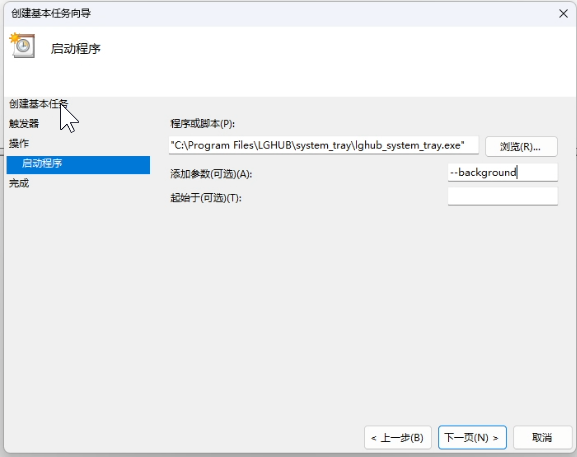
\includegraphics[width=\textwidth]{docs/assets/skills/create_basic_task_06.png}
    \caption{添加 \lstinline{--background} 参数}
\end{figure}

勾选图示选项后,点击完成。

\begin{figure}[H]
    \Centering
    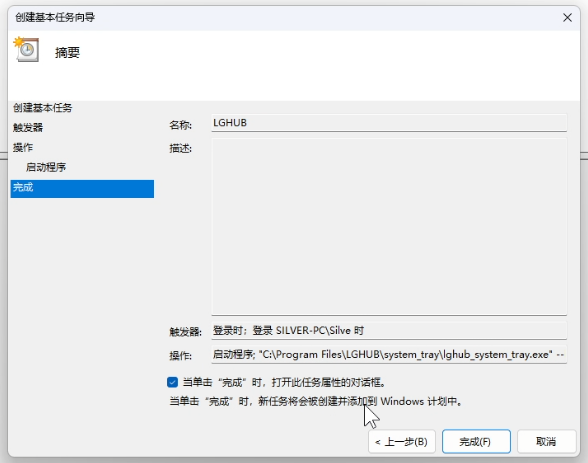
\includegraphics[width=\textwidth]{docs/assets/skills/create_basic_task_07.png}
    \caption{完成后弹出任务属性对话框}
\end{figure}

在弹出的窗口中选择“使用最高权限运行”。

\begin{figure}[H]
    \Centering
    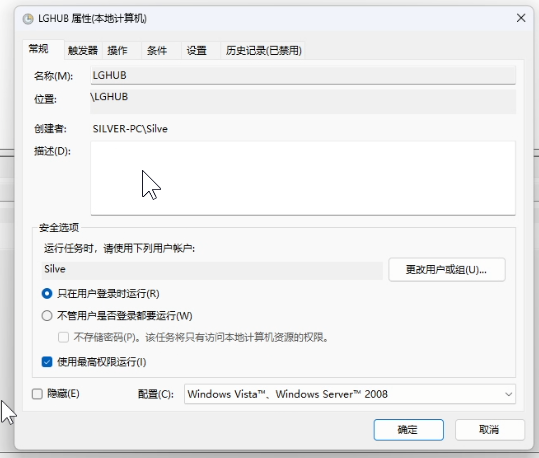
\includegraphics[width=\textwidth]{docs/assets/skills/create_basic_task_08.png}
    \caption{勾选“使用最高权限运行”}
\end{figure}

然后,点击“条件”,去除下图所示的与电源相关的任务运行条件\textbf{\color{red}(对于笔记本用户,此项必须去除,否则在笔记本使用电池电源时,任务将不会启动,启动的任务也将退出)}。

\begin{figure}[H]
    \Centering
    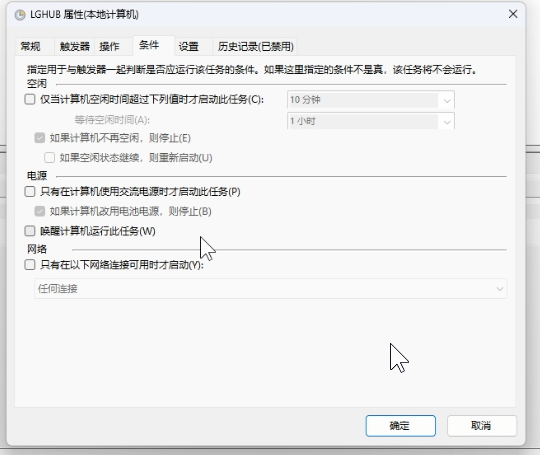
\includegraphics[width=\textwidth]{docs/assets/skills/create_basic_task_09.png}
    \caption{去除与电源相关的任务运行条件}
\end{figure}

最后,点击“设置”,去除与程序运行时间限制(如“运行时间超过 3 天停止任务”这样的选项)。

\begin{figure}[H]
    \Centering
    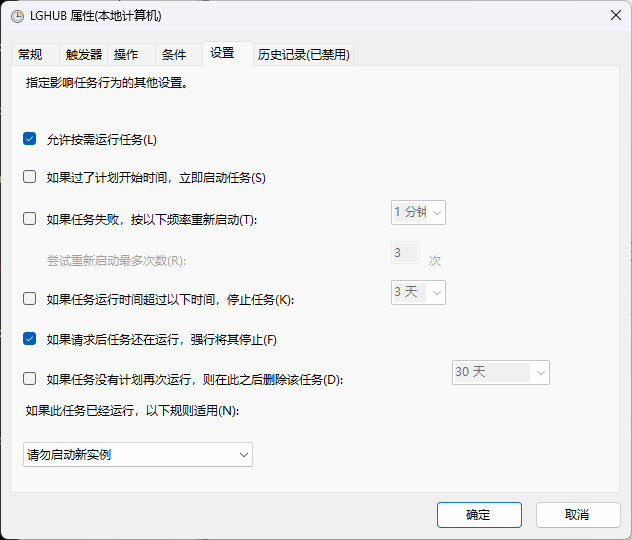
\includegraphics[width=\textwidth]{docs/assets/skills/create_basic_task_10.png}
    \caption{解除运行时间限制}
\end{figure}

点击“确定”后,可在 \lstinline{LGHUB} 文件夹中找到新创建的基本任务。下一次电脑开机并以当前用户账户登录后,罗技软件将自动以管理员权限启动。

\begin{figure}[H]
    \Centering
    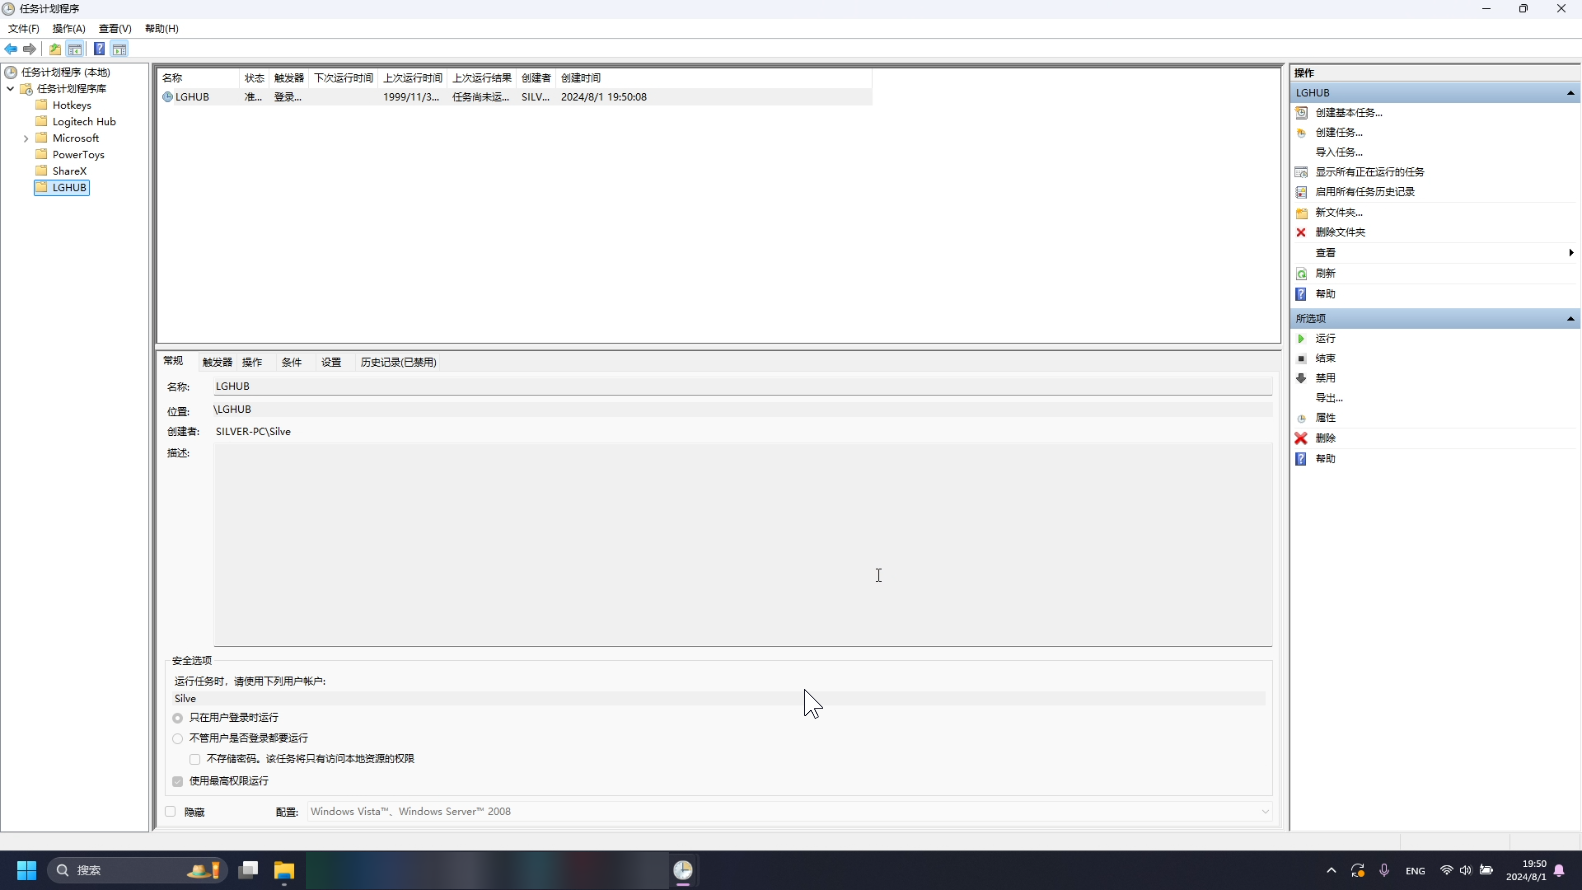
\includegraphics[width=\textwidth]{docs/assets/skills/create_basic_task_11.png}
    \caption{创建完成的基本任务}
\end{figure}

要想立即运行已经创建的基本任务,请右键该任务,点击“运行”即可(已经运行则跳过此步骤)。上述创建开机自启任务的方法同样适用于其他任何应用程序。

\begin{figure}[H]
    \Centering
    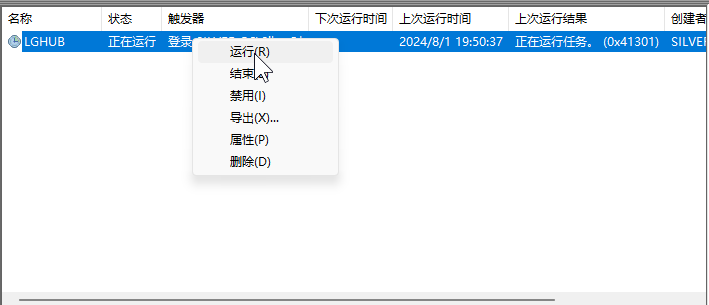
\includegraphics[width=\textwidth]{docs/assets/skills/run_task.png}
    \caption{立即运行已经创建的基本任务}
\end{figure}


\subsection{使用模式 2 抢杀敌 MVP}
\label{subsection-mode-2-skill-0}

如果您拥有逆界星轮,则可以考虑\textbf{在无限制挂机房挂机时}使用模式 2 抢夺杀敌 MVP。配置方式如下(仅供参考,购买按键序列需要自行修改),只需要在随机武器列表中保留一件逆界星轮即可。

\begin{minted}[breakautoindent, breaklines]{lua}
---扩展武器列表。
---@type Weapon[]
ExtendedWeaponList = {
    Weapon:new{
        name = "逆界星轮",
        switch_delay = Delay.NORMAL,
        number = Weapon.PRIMARY,
        purchase_sequence = {Keyboard.B, Keyboard.EIGHT, Keyboard.SIX},
        attack_button = Mouse.RIGHT
    }
}
\end{minted}

这样,在扩展挂机模式下,游戏开始的前 120 秒使用默认挂机模式积攒充足资金后,便会持续进行逆界星轮刷枪操作,其杀敌效率远超【青鸾】迅风轮等武器。若您还拥有圣翼皓印或炽翼魔印,则配合样例文件中提供的特殊武器使用方式,还可进一步提升杀敌效率。

\subsection{使用模式 2 刷狂戮巨蚊、鹞子风筝任务}
\label{subsection-mode-2-skill-1}

在拥有【天驱】突击套装、【擎空】突击套装、冰雪魔咒 PB-4 其中之一的情况下,可以使用模式 2 刷狂戮巨蚊、鹞子风筝任务。

这需要您对随机武器列表作如下配置(仅供参考,购买按键序列需要自行修改)。鉴于【天驱】突击套装、【擎空】突击套装没有吸血效果,故在随机武器列表额外加入幻境!光棱剑。

\begin{minted}[breakautoindent, breaklines]{lua}
---扩展武器列表。
---@type Weapon[]
ExtendedWeaponList = {
    Weapon:new{
        name = "幻境!光棱剑",
        switch_delay = Delay.NORMAL,
        number = Weapon.MELEE,
        purchase_sequence = {Keyboard.B, Keyboard.G},
        attack_button = Mouse.LEFT
    },
    Weapon:new{
        name = "【擎空】突击套装",
        switch_delay = Delay.NORMAL,
        number = Weapon.SECONDARY,
        purchase_sequence = {Keyboard.B, Keyboard.ONE, Keyboard.ONE},
        attack_button = Mouse.LEFT
    },
    Weapon:new{
        name = "【天驱】突击套装",
        switch_delay = Delay.NORMAL,
        number = Weapon.SECONDARY,
        purchase_sequence = {Keyboard.B, Keyboard.ONE, Keyboard.TWO},
        attack_button = Mouse.LEFT
    },
    Weapon:new{
        name = "冰雪魔咒PB-4",
        switch_delay = Delay.NORMAL,
        number = Weapon.SECONDARY,
        purchase_sequence = {Keyboard.B, Keyboard.ONE, Keyboard.THREE},
        attack_button = Mouse.LEFT
    }  attack_button = Mouse.RIGHT
}
\end{minted}

需要指出,随机武器列表中的武器是等概率随机选择的,若要提高某一件武器被选中的概率,只需要在武器列表中多次添加改武器即可(重复添加同一件武器时,其名称需要保持相同,否则将被认为是不同的武器,Lua 模块针对重复购买相同武器刷枪的情况有特别优化)。
例如,刷狂戮巨蚊、鹞子风筝任务时,若您只有【天驱】突击套装(签到可免费领取),要提高【天驱】突击套装被选中的概率(上面的例子中被选中的概率为 25\%),只需要进行下面这样的改动,即可将【天驱】突击套装被选中的概率提高到 75\%。

\begin{minted}[breakautoindent, breaklines]{lua}
---扩展武器列表。
---@type Weapon[]
ExtendedWeaponList = {
    Weapon:new{
        name = "幻境!光棱剑",
        switch_delay = Delay.NORMAL,
        number = Weapon.MELEE,
        purchase_sequence = {Keyboard.B, Keyboard.G},
        attack_button = Mouse.LEFT
    },
    Weapon:new{
        name = "【天驱】突击套装",
        switch_delay = Delay.NORMAL,
        number = Weapon.SECONDARY,
        purchase_sequence = {Keyboard.B, Keyboard.ONE, Keyboard.TWO},
        attack_button = Mouse.LEFT
    },
    Weapon:new{
        name = "【天驱】突击套装",
        switch_delay = Delay.NORMAL,
        number = Weapon.SECONDARY,
        purchase_sequence = {Keyboard.B, Keyboard.ONE, Keyboard.ONE},
        attack_button = Mouse.LEFT
    },
    Weapon:new{
        name = "【天驱】突击套装",
        switch_delay = Delay.NORMAL,
        number = Weapon.SECONDARY,
        purchase_sequence = {Keyboard.B, Keyboard.ONE, Keyboard.TWO},
        attack_button = Mouse.LEFT
    }  attack_button = Mouse.RIGHT
}
\end{minted}

根据实测效果,使用模式 2 进行如上配置后单刷狂戮巨蚊仅需一天。

\subsection{远程控制挂机}

本工具可结合贝锐™向日葵等远程控制软件使用,实现远程控制挂机的效果。具体使用方法超出本手册讨论范畴,故不在本手册中进行介绍。